

\begin{lemma}[Table of Laplace Transforms]\label{ec/2010/41/tbl}
\begin{center}
\begin{tabular}{ |m{3cm}|m{4.5cm}| } 
 \hline
 $\textbf{Time Function}$ $f(t)=\mathcal{L}^{-1}\cbrak{F(s)}$ & $\textbf{Laplace transform}$ of f(t) $F\brak{s}=\mathcal{L}\cbrak{f\brak{t}}$ \\ 
 \hline
 $u\brak{t}$ & $\frac{1}{s}$, $s>0$ \\ 
 \hline
 $g^{\prime}(t)$ & $sG\brak{s}-g(0)$ \\ 
 \hline
 $g^{\prime\prime}\brak{t}$ & $s^2G\brak{s}-sg\brak{0}-g^{\prime}\brak{0}$\\
 \hline
 $e^{-at}u\brak{t}$ & $\frac{1}{s+a}$, $s+a>0$\\
 \hline
\end{tabular}
\end{center}
\end{lemma}
\begin{lemma}{Linearity of Laplace Transform}
\begin{align}
    \mathcal{L}\cbrak{af\brak{t}+bg\brak{t}}=a\mathcal{L}\cbrak{f\brak{t}}+b\mathcal{L}\cbrak{g\brak{t}}
\end{align}
\end{lemma}
From Lemma-\ref{ec/2010/41/tbl} Laplace transform of $x\brak{t}=e^{-2t}u\brak{t}$ is given by
\begin{align}
    X\brak{s}=\frac{1}{s+2}
\end{align}
Since initial conditions are zero. Laplace Transform of $\eqref{ec/2010/41/q}$ gives
\begin{align}
    s^{2}Y\brak{s}+4sY\brak{s}+3Y\brak{s}&=2sX\brak{s}+4X\brak{s}\\
    Y\brak{s}&=\frac{2\brak{s+2}}{s^2+4s+3}X\brak{s}\\
    &=\frac{1}{s+1}-\frac{1}{s+3}
\end{align}
From Lemma-$\ref{ec/2010/41/tbl}$. Inverse Laplace transform of $Y\brak{s}$ is given by
\begin{align}
    y(t)&=e^{-t}u\brak{t}-e^{-3t}u\brak{t}\\
    &=\brak{e^{-t}-e^{-3t}}u\brak{t}
\end{align}
$\therefore$ The required option is B.  See Fig. \ref{ec/2010/41/fig/}.
\
\begin{figure}[!h]
 \centering
 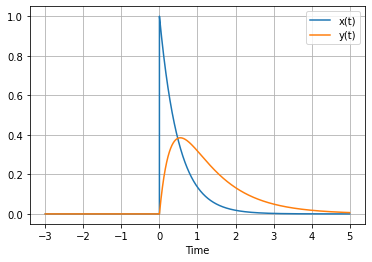
\includegraphics[width=\columnwidth]{solutions/ec/2010/41/figs/plt.png}
 \caption{Plot of input and output responses in time domain.}
 \label{ec/2010/41/fig/}
\end{figure}

